%%
%% Class homework & solution template for latex
%% Alex Ihler
%%
\documentclass[twoside,11pt]{article}
\usepackage{amsmath,amsfonts,amssymb,amsthm}
\usepackage{graphicx,color}
\usepackage{verbatim,url}
\usepackage{listings}
\usepackage{subcaption} 
\usepackage{upquote}
\usepackage[T1]{fontenc}
%\usepackage{lmodern}
\usepackage[scaled]{beramono}
%\usepackage{textcomp}

% Directories for other source files and images
\newcommand{\bibtexdir}{../bib}
\newcommand{\figdir}{fig}

\newcommand{\E}{\mathrm{E}}
\newcommand{\Var}{\mathrm{Var}}
\newcommand{\N}{\mathcal{N}}
\newcommand{\matlab}{{\sc Matlab}\ }

\setlength{\textheight}{9in} \setlength{\textwidth}{6.5in}
\setlength{\oddsidemargin}{-.25in}  % Centers text.
\setlength{\evensidemargin}{-.25in} %
\setlength{\topmargin}{0in} %
\setlength{\headheight}{0in} %
\setlength{\headsep}{0in} %

\renewcommand{\labelenumi}{(\alph{enumi})}
\renewcommand{\labelenumii}{(\arabic{enumii})}

\theoremstyle{definition}
\newtheorem{MatEx}{M{\scriptsize{ATLAB}} Usage Example}

\definecolor{comments}{rgb}{0,.5,0}
\definecolor{backgnd}{rgb}{.95,.95,.95}
\definecolor{string}{rgb}{.2,.2,.2}
\lstset{language=Matlab}
\lstset{basicstyle=\small\ttfamily,
        mathescape=true,
        emptylines=1, showlines=true,
        backgroundcolor=\color{backgnd},
        commentstyle=\color{comments}\ttfamily, %\rmfamily,
        stringstyle=\color{string}\ttfamily,
        keywordstyle=\ttfamily, %\normalfont,
        showstringspaces=false}
\newcommand{\matp}{\mathbf{\gg}}




\begin{document}

\centerline{\Large Homework 2}
\centerline{Zachary DeStefano, 15247592}
\centerline{CS 274B: Spring 2016}

\section*{Problem 1: }

\subsection*{Part A,B}

Here is the code I used to produce the mutual information
\begin{lstlisting}
#Part A
D = np.genfromtxt('data/data.txt',delimiter=None)
loc = np.genfromtxt('data/locations.txt',delimiter=None)
m,n = D.shape # m = 2760 data points, n=30 dimensional

#Part B

#Find phat for each variable
posXcount = np.sum(D,axis=0)
probXj = np.zeros((n,2))
probXj[:, 1] = np.divide(posXcount,m)
probXj[:, 0] = 1-probXj[:,1]

#Find phat(x_j,x_k) for each pair of variables
probXjk = np.zeros((n,n,2,2))
for i in range(n):
    for j in range(n):
        for k in range(m):
            probXjk[i, j, D[k, i], D[k, j]] += 1
probXjk = np.divide(probXjk,m)

#Compute mutual information
mutualInfo = np.zeros((n,n))
for i in range(n):
    for j in range(n):
        curTerm = 0
        for k1 in range(2):
            for k2 in range(2):
                denomTerm = probXj[i,k1]*probXj[j,k2]
                jointTerm = probXjk[i, j, k1, k2]
                if denomTerm>0 and jointTerm>0:
                    curTerm += jointTerm*np.log(jointTerm/denomTerm)
        mutualInfo[i, j] = curTerm

#print results
print mutualInfo[0:5,0:5]
\end{lstlisting}

Here are the first 5 rows and columns of mutual information
\begin{lstlisting}
[[ 0.60870002  0.24584358  0.30645904  0.17521613  0.24642811]
 [ 0.24584358  0.66081843  0.28479996  0.21222061  0.29414659]
 [ 0.30645904  0.28479996  0.64609051  0.21486084  0.27873285]
 [ 0.17521613  0.21222061  0.21486084  0.68239551  0.23489376]
 [ 0.24642811  0.29414659  0.27873285  0.23489376  0.67286449]]
\end{lstlisting}
\newpage
\subsection*{Part C}

For the algorithm, I added edges in descending order by weight if they did not make a cycle. To compute this, I first initialized the edge information arrays:
\begin{lstlisting}
edges = np.zeros(n*(n-1)/2)
edgeNodeID = np.zeros((n*(n-1)/2,2))
edgeInd = 0
for i in range(n):
    for j in range(i+1,n):
        edges[edgeInd] = mutualInfo[i, j]
        edgeNodeID[edgeInd,:] = [i, j]
        edgeInd+=1

sortedEdges = np.sort(edges)[::-1]
sortedEdgeID = np.argsort(edges)[::-1]
\end{lstlisting}

I made a function \textit{nodesHavePath} that tells whether an edge will form a cycle
\begin{lstlisting}
def nodesHavePath(adjMatrix,node0,node1):

    n,m = adjMatrix.shape
    adjMatrix = adjMatrix + np.transpose(adjMatrix)
    adjPower = np.copy(adjMatrix)
    adjTotal = np.copy(adjMatrix)
    for i in range(n):
        adjPower = np.dot(adjMatrix, adjPower)
        adjTotal += adjPower

    return (adjTotal[node0,node1]>0)
\end{lstlisting}

I then computed the adjacency matrix for the Chow-Liu Tree:
\begin{lstlisting}
adjMatrix = np.zeros((n,n))
for curI in range(len(sortedEdges)):
    curEdgeID = sortedEdgeID[curI]
    curNode0 = edgeNodeID[curEdgeID, 0]
    curNode1 = edgeNodeID[curEdgeID, 1]
    if not nodesHavePath(adjMatrix,curNode0,curNode1):
        adjMatrix[curNode0,curNode1]=1
\end{lstlisting}

\newpage

To print the edges, I made an adjacency list that does not repeat edges. Here is the code that makes the list and prints out the results
\begin{lstlisting}
def getAdjList(adjMatrix):
    mm,xx = adjMatrix.shape
    visited = np.zeros((mm))
    adjList = []
    listVertices = []
    for i in range(mm):
        visited[i] = 1
        adjVertices = np.where(adjMatrix[i,:]>0)
        verticesAdd = []
        for j in adjVertices[0]:
            if visited[j] <= 0:
                verticesAdd.append(j)
        if len(verticesAdd) > 0:
            adjList.append(verticesAdd)
            listVertices.append(i)
    return listVertices,adjList

listVertices,adjList = getAdjList(adjMatrix)
for i in range(len(listVertices)):
    print listVertices[i],adjList[i]
\end{lstlisting}

Here is the printed result
\begin{lstlisting}
0 [2]
1 [4]
2 [16, 17]
3 [5, 12, 29]
4 [6]
5 [6]
7 [10, 13]
8 [13]
9 [10]
10 [14]
11 [12, 14]
13 [15]
17 [18, 20]
18 [19]
20 [27]
21 [24, 25, 27]
22 [23, 26, 28]
27 [29]
28 [29]
\end{lstlisting}
\newpage
Here is the code I used to produce the graph drawing of the Chow-Liu Tree
\begin{lstlisting}
graph2 = nx.Graph()
graph2.add_nodes_from(range(n))
for i in range(len(listVertices)):
		for j in adjList[i]:
				graph2.add_edge(listVertices[i],j)
loc2 = np.zeros(loc.shape)
loc2[:, 0] = loc[:, 1]
loc2[:, 1] = loc[:, 0]
nx.draw_networkx(graph2, node_color='c', pos=loc2)
plt.title('Weather Station Locations with Chow-Liu Tree')
plt.xlabel('Longitude')
plt.ylabel('Latitude')
plt.show()
\end{lstlisting}

\begin{figure}[h]
\centering
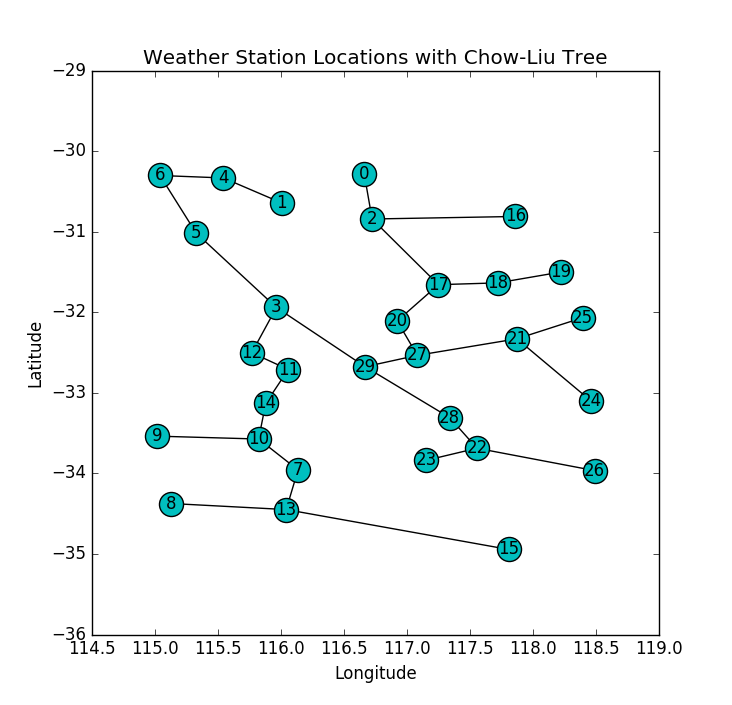
\includegraphics[width=6in]{chowLiuTreeFigure2.png}
\caption{Chow-Liu Tree as computed in Part C}
\end{figure}

\subsection*{Part D}

To calculate the likelihood, I used the method in Slide 6 of \textit{Structure Learning in Bayes Nets} where you add together the entropy and mutual information. Here is the code:
\begin{lstlisting}

#look at diagnoal of mutual info matrix for entropy
mutualInfoEntropy = np.zeros(n)
for i in range(n):
    mutualInfoEntropy[i] = mutualInfo[i,i]
entropyPart = mutualInfoEntropy.sum()

mutualInfoPart = 0
for jj in range(len(listVertices)):
    curJind = listVertices[jj]
    for kk in adjList[jj]:
        mutualInfoPart += mutualInfo[curJind,kk]

loglike = mutualInfoPart - entropyPart

print 'Log Likelihood:'
print loglike
\end{lstlisting}

Here is the result
\begin{lstlisting}
Log Likelihood:
-11.0986143278
\end{lstlisting}

\newpage

\section*{Problem 2:}

\subsection*{Part A}

Here is the loopy model compared with the Chow-Liu Tree Model. The loopy model seems more logical because it resembles a real-world network slightly better. 

\begin{figure}[h]
\centering
\begin{subfigure}{.5\textwidth}
  \centering
  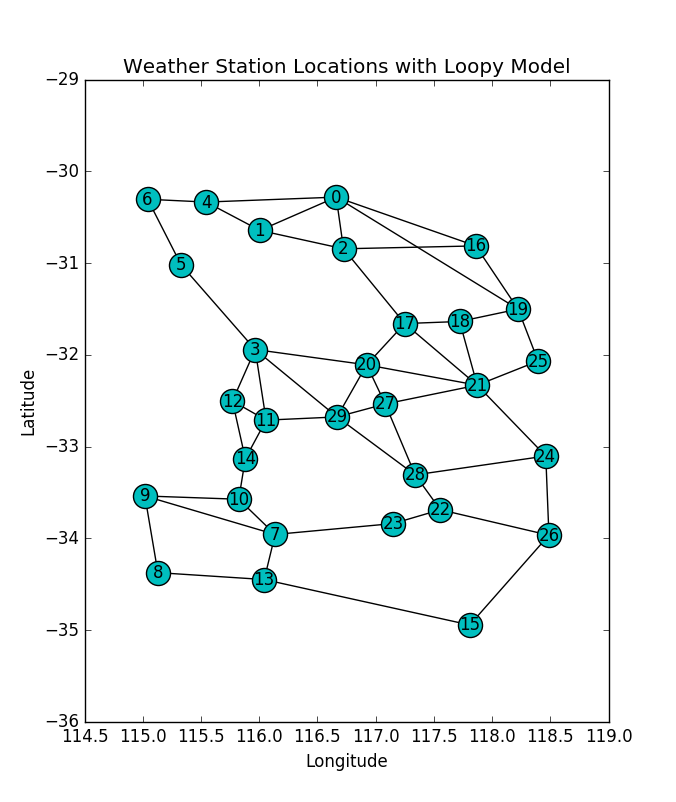
\includegraphics[width=3 in]{loopyModelFigure2.png}
  \caption{Loopy Model}
\end{subfigure}%
\begin{subfigure}{.5\textwidth}
  \centering
  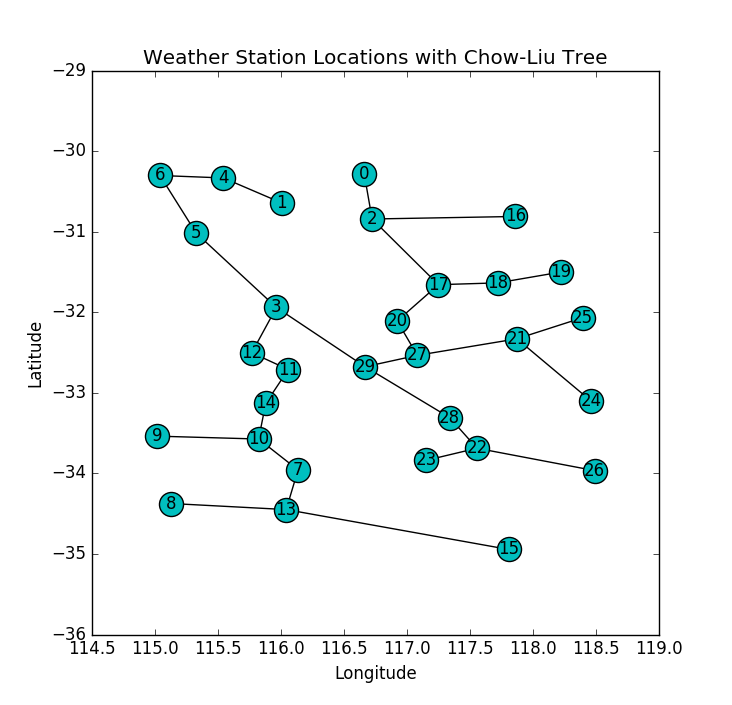
\includegraphics[width=3 in]{chowLiuTreeFigure2.png}
  \caption{Chow-Liu Tree Model}
\end{subfigure}
\caption{Loopy Model and Chow-Liu Tree Model side-by-side}
\end{figure}

\newpage

\subsection*{Part B}

Here is the code for the empirical marginal probabilities
\begin{lstlisting}
#this find phat for each variable
posXcount = np.sum(D,axis=0)
probXj = np.zeros((n,2))
probXj[:, 1] = np.divide(posXcount,m)
probXj[:, 0] = 1-probXj[:,1]

#this find phat(x_j,x_k) for each pair of variables
# next dimension is probability of j, then prob of k
probXjk = np.zeros((n,n,2,2))
for i in range(n):
    for j in range(n):
        for k in range(m):
            probXjk[i, j, D[k, i], D[k, j]] += 1
probXjk = np.divide(probXjk,m)

#find phat(x_j|x_k)
probXjGivenK = np.zeros((n,n,2,2))
for i in range(n):
    for j in range(n):
        for jval in range(2):
            for kval in range(2):
                probXjGivenK[i,j,jval,kval] = probXjk[i,j,jval,kval]/probXj[j,kval]

def getAdjList(adjMatrix):
    mm,xx = adjMatrix.shape
    visited = np.zeros((mm))
    adjList = []
    listVertices = []
    for i in range(mm):
        visited[i] = 1
        adjVertices = np.where(adjMatrix[i,:]>0)
        verticesAdd = []
        for j in adjVertices[0]:
            if visited[j] <= 0:
                verticesAdd.append(j)
        if len(verticesAdd) > 0:
            adjList.append(verticesAdd)
            listVertices.append(i)
    return listVertices,adjList

listVertices,adjList = getAdjList(adjMatrix)

\end{lstlisting}

TODO: PRINT OUT RESULTS

\subsection*{Part C}

TODO: COMMENT THE CODE, DETAIL ITS PARTS MORE, AND INPUT THE RESULTING FIGURE

\begin{lstlisting}
gmNodes = [gm.Var(i,2) for i in range(n)]
probNodes = [gm.Var(i,2) for i in range(n)]
#print gmNodes

#makes the factors given the loopy model graph we have
gmFactors = []
probFactors = []
for jj in range(len(listVertices)):
    curJind = listVertices[jj]
    for kk in adjList[jj]:
        gmFactors.append(gm.Factor([gmNodes[curJind],gmNodes[kk]],1.0))
        probFactors.append(gm.Factor([probNodes[curJind], probNodes[kk]], 1.0))

#fills the table with the empiricial probabilities we have calculated
curListInd = 0
for jj in range(len(listVertices)):
    curJind = listVertices[jj]
    for kk in adjList[jj]:
        #inputFactor = np.matrix(np.ones((3,3))) ; # TEST CODE
        inputFactor = np.matrix(np.ones((2, 2)))
        #inputFactor = np.multiply(inputFactor,0.25)
        gmFactors[curListInd].table = inputFactor
        probFactors[curListInd].table = probXjk[curJind,kk,:,:]
        curListInd += 1


sumElim = lambda F,Xlist: F.sum(Xlist)   # helper function for eliminate

numIter=6
logLikeIter = np.zeros(numIter)
for iterI in range(numIter):
    print 'Now computing Iteration: ',iterI
    listInd = 0
    for jj in range(len(listVertices)):
        curJind = listVertices[jj]
        for kk in adjList[jj]:
            #print jj,kk

            #does variable elimination to get p_ij value
            currentFactors = copy.deepcopy(gmFactors)
            curModel = gm.GraphModel(currentFactors)
            pri = [1.0 for Xi in currentFactors]
            pri[curJind], pri[kk] = 2.0, 2.0
            order = gm.eliminationOrder(curModel,orderMethod='minfill',priority=pri)[0]
            curModel.eliminate(order[:-2], sumElim)  # eliminate all but last two
            curP = curModel.joint()
            curLnZ = np.log(curP.sum())
            #print 'lnZ: ', curLnZ
            curP /= curP.sum()
            #print curP.table

            curLog = 0
            probModel = gm.GraphModel(probFactors)
            for ptNum in range(m):
                curLog += probModel.logValue(D[ptNum,:])
            curLog = curLog/m
            #print 'logLike: ',curLog/m,'\n'

            #update the factor
            currentFij = gmFactors[listInd].table
            probRatio = np.matrix(np.divide(probXjk[curJind,kk,:,:],curP.table))
            newFij = np.multiply(currentFij,probRatio)
            gmFactors[listInd].table = newFij

            newFijNorm = newFij/newFij.sum()
            probFactors[listInd].table = newFijNorm

            listInd+=1
    logLikeIter[iterI] = curLog

plt.plot(logLikeIter)
plt.show()

\end{lstlisting}

\end{document}
